\newcommand{\upcite}[1]{\textsuperscript{\textsuperscript{\cite{#1}}}}
\chapter*{\zjutitlec 中期报告}

\section{项目背景}
原始神经元图像信息的神经元追踪和数字重建是神经科学界热门方向。神经元的形态反应出它的功能,相同功能的神经元通常具有类似的功能。神经科学家通过结构脑图谱的重建,可以反推大脑是如何运作,对理解智慧的产生有重要的帮助。Cannon RC 等人在海马神经重建上做出的工作\upcite{Cannon1998An},Feng L 等人使用 mGRASP 在鼠类大脑上进行的重建工作\upcite{Druckmann2014Structured}均取得了出色的进展。

由于神经元拓扑结构的复杂性,在一些自动化重建结果的细节上仍然需要研究人员对数字重建的结果进行人工纠正和修改,以确保数字重建工作的准确性。另外研究人员需要对数字重建结果进行编辑,比如添加或删除一些网络分支等。为了便于研究人员编辑数字重建的结果,根据“所见即所得”的原则,设计出了 SWC 格式\upcite{Peng2011Proof}。SWC 框架有以下特征: 清楚的 SWC 结构以及原始数据参考的可视化,明确定义的可操作单元,以及将用户输入和编辑操作直观地对应起来。在 SWC 格式的基础上,研究人员可以方便、直观地纠正自动化数字重建结果的错误,添加新的分支或删除已有分支。Feng,Linqing, Zhao Ting, Kim Jinhyun 等人\upcite{Feng2014neuTube}充分充分发挥了 SWC 格式高效,精确的优点,提供了同时在 2D 和 3D 模式下查看,编辑神经元结构的功能。

由于 neuTube 是运行在单机的软件,无法满足多用户协同编辑修改的需求,也不利于结构脑图谱的交流。随着计算机性能和网络速度的提升,在线实时编辑神经元网络结构成为了可能。在此背景下,我们希望设计并实现一个在线多用户的神经元网络结构编辑分享平台,利用互联网便于数据共享的特点,帮助神经学研究人员便捷地进行异地,多用户协同编辑神经元网络结构,并能分享结构脑图谱,共同探索神经元结构下的奥秘。

\section{整体架构}
项目整体结构如图 \ref{server} 所示,共分为神经信息数据库,用户信息数据库以及网络服务器三部分组成。
\begin{figure}
\centering
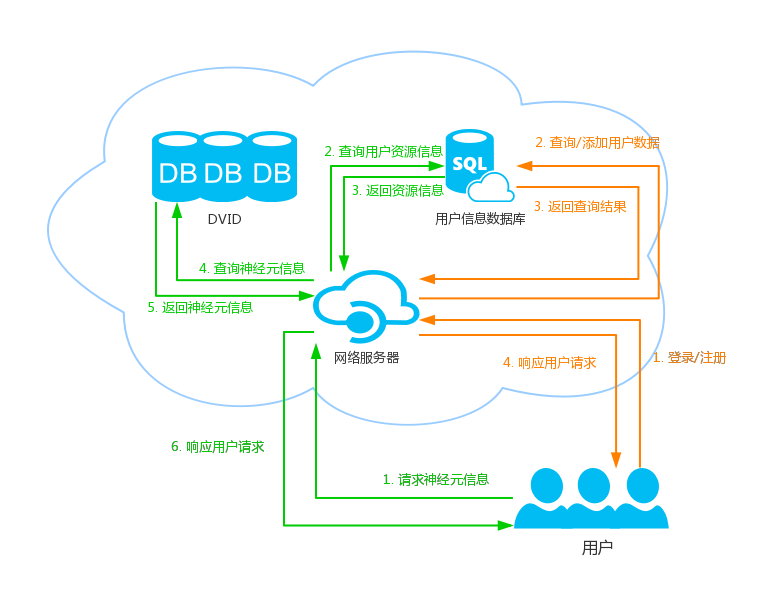
\includegraphics[width=148mm]{images/server}
\caption{项目整体架构}
\label{server}
\end{figure}

\subsection{神经信息数据库}
神经信息数据库包含两部分数据,一部分是原始大脑切片显微镜图像,另外一部分是初步完成数字重建的 SWC 文件。使用 DVID 作为数据库,储存这些信息。DVID 是一个分布式面向图像的数据服务,主要用于图像分析与可视化。DVID 有如下特点:

1. 便于扩展数据类型,允许用户根据数据特点加速访问速度,减少储存空间,提供方便的 API。这为储存数字重建结果提供了便利。

2. 为分布式数据储存提供了类似于 GIT 的版本控制系统,在此基础之上我们可以解决多用户同时编辑产生冲突的问题。

3. 方便连接其他 API 如 Google BrainMaps 和 OpenConnectome 等。

4. 支持多分辨率图像数据,使得用户可以在不同尺度下观察图像信息。

在 DVID 的基础上,构建出原始大脑切片显微镜图像与数字重建结果的储存仓库,将数据储存抽象成数据存储服务,使得可以专注于完成核心算法和逻辑。

\subsection{用户信息数据库}
用户信息数据库包含多用户管理以及用户资源管理。使用 PostgreSQL 数据库储存这部分信息。PostgreSQL 最初由加州大学伯克利分校计算机系开发完成。在支持大部分 SQL 标准之上,提供了许多诸如复杂查询,多版本并行控制,事物完整性等现代特性\upcite{stonebraker1991postgres}。由于 PostreSQL 对标准 SQL 支持度较高,可以方便的和 DVID 联系起来,将用户信息和原始图像信息,数字重建结果对应起来。利用 PostgreSQL 支持的储存过程,事物以及多版本并行控制特性,我们可以方便的实现分布式,多用户实时编辑平台,并解决多用户同时编辑可能产生冲突的问题。

\subsubsection{数据表设计}
为了实现多用户管理以及用户资源管理,共设计实现了三张数据表,分别是用户信息表,原始图像数据表以及 swc 数据表。

1. 用户信息表
用户信息表如表 \ref{user-table} 所示,共有三个字段,分别储存了用户名,密码和用户保证账户安全的盐值。
\begin{table}
\centering
\caption{用户信息表}
\begin{tabular}{|c|c|c|}
			   \hline
                 字段名 & 数据类型 & 备注 \\
               \hline
                 username & STRING & 主键 \\
               \hline
                 password & STRING &  \\
               \hline
                 salt & UUID & 用于保证用户账户安全 \\
               \hline
             \end{tabular}
             \label{user-table}    
\end{table}

2. 原始图像数据表
原始图像数据表如表 \ref{image-table} 所示,共有三个字段,分别储存了创建者,图像名和权限控制的用户角色。

\begin{table}
\centering
\caption{原始图像数据表}
\begin{tabular}{|c|c|c|}
			   \hline
                 字段名 & 数据类型 & 备注 \\
               \hline
                 username & STRING & 创建者,外键,用户信息表中的 username \\
               \hline
                 image & STRING &  \\
               \hline
                 role & STRING & 用于权限控制 \\
               \hline
             \end{tabular}
             \label{image-table}    
\end{table}

3. swc 数据表
原始图像数据表如表 \ref{swc-table} 所示,共有五个字段,分别储存了创建者,图像名,创建时间,swc 文件名以及用户评论。根据创建时间,可以建立同一图像下 swc 文件的拓扑顺序,为多用户同时编辑以及合并冲突分支提供了基础。

\begin{table}
\centering
\caption{原始图像数据表}
\begin{tabular}{|c|c|c|}
			   \hline
                 字段名 & 数据类型 & 备注 \\
               \hline
                 username & STRING & 创建者,外键,用户信息表中的 username \\
               \hline
                 image & STRING & 原始图像名,外键,原始图像数据表中的 image \\
               \hline
                 createdAt & TIME & 创建时间 \\
               \hline
                 swc & TEXT & swc 文件名 \\
               \hline
                 comments & STRING & 备注 \\
               \hline
             \end{tabular}
             \label{swc-table}    
\end{table}

\subsubsection{网络服务器}


\section{性能测试}
为了提供一个高可用的实时编辑功能,需要能对用户的操作迅速做出反应,降低响应延迟。使用 Gatling 作为压力测试工具,进行了压力测试。如图 \ref{overview} 所示,在 5 分钟的时间里进行了 31000 次请求,下文做更加详细的分析。
\begin{figure}
\centering
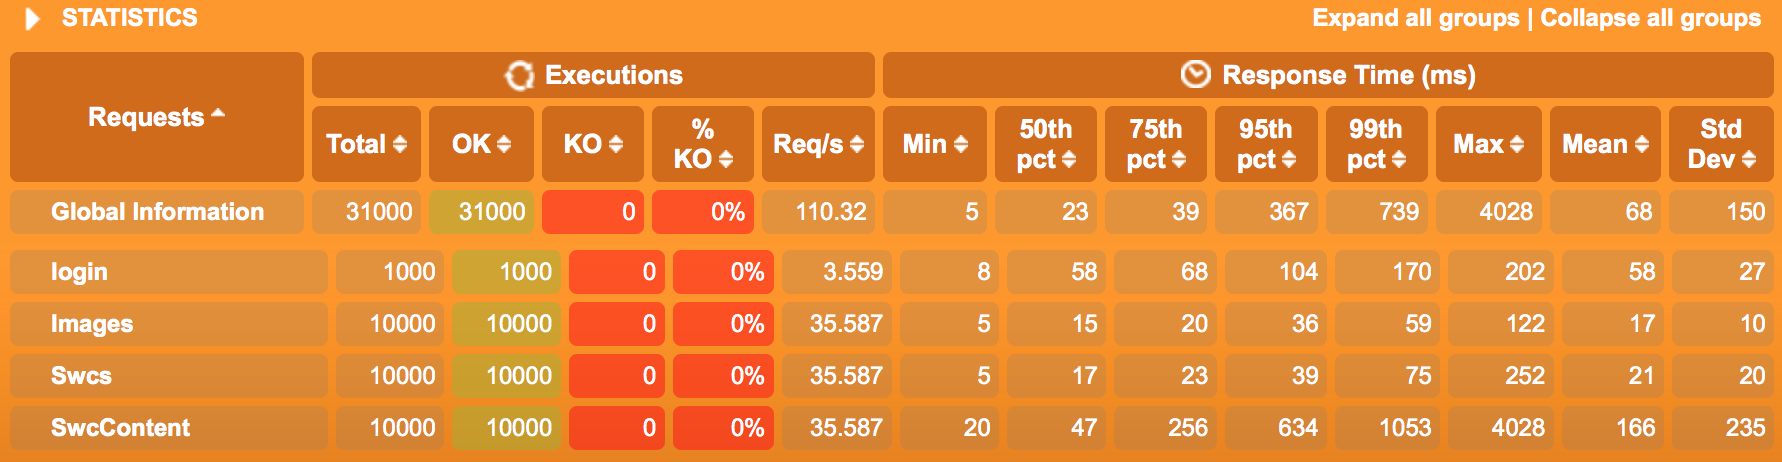
\includegraphics[width=148mm]{images/overview}
\caption{压力测试概述}
\label{overview}
\end{figure}

\subsection{响应时间分析}

Grigorik 通过分析大量用户数据提出用户能明显感受到毫秒级别的延迟,即使平时生活中接触不到毫秒级别的时间。延迟在 100ms 以内的时候,用户会认为立即得到了响应;在 100 ~ 300 ms 之间,用户会感觉到轻微的延迟;300 ~ 1000 ms 之间,用户仅仅认为系统工作正常,但体验较差;当延迟达到 1000 ms 之上的时候,用户会去做其他工作;如果延迟达到了 10 000ms 的时候,用户便放弃这项任务\upcite{grigorik2013high}。 

在图 \ref{response} 和图 \ref{overview} 中可以看出,最低响应时间为 5 ms, 最高响应时间为 4028 ms, 平均响应时间为 68 ms。绝大多数请求的响应时间在 100ms 以下,少部分请求响应时间在 100~400 ms 之间,极少数请求的响应时间在 1000 ms 以上。在图 \ref{overtime} 可以看出不同响应时间的请求占总请求比例随时间变化趋势。按照 Grigorik 的标准,基本满足了实时操作的要求。

\begin{figure}
\centering
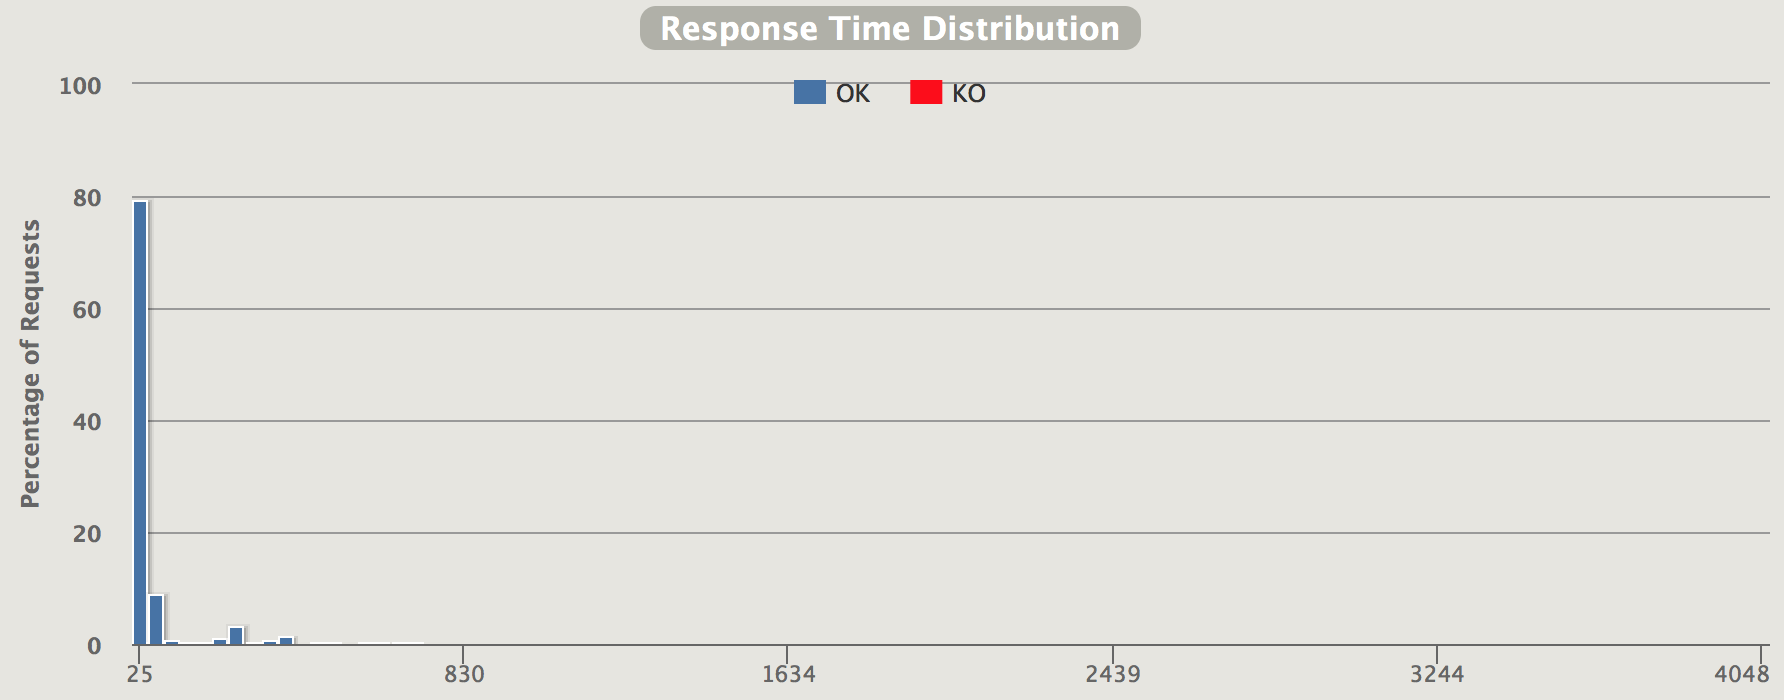
\includegraphics[width=148mm]{images/response}
\caption{响应时间}
\label{response}
\end{figure}

\begin{figure}
\centering
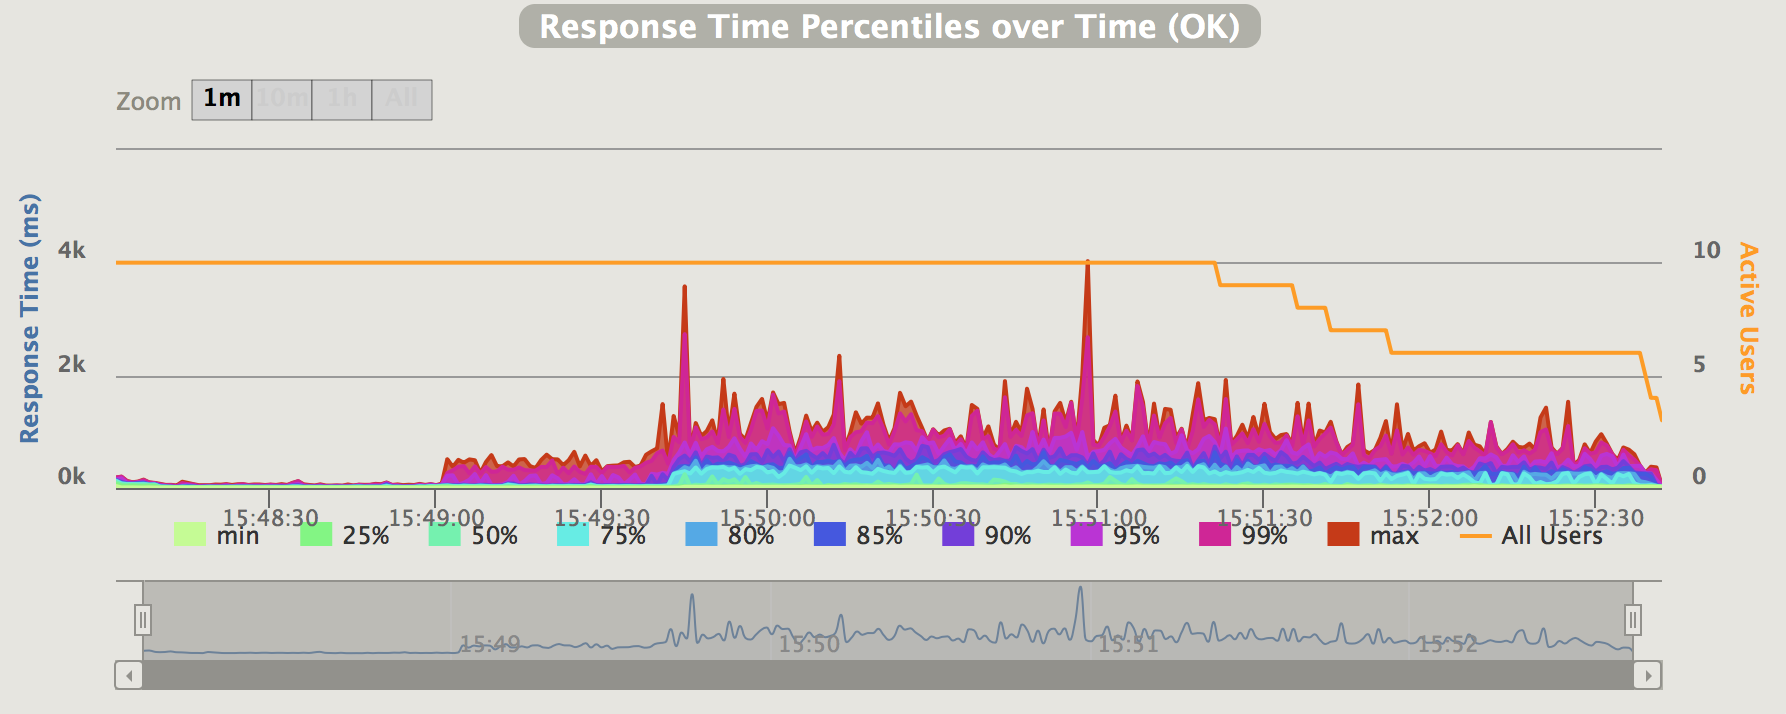
\includegraphics[width=148mm]{images/overtime}
\caption{不同响应时间的请求随时间变化趋势}
\label{overtime}
\end{figure}

\subsection{并发请求分析}
在图 \ref{request} 中描述了网络服务器处理请求的数量随着时间变化的趋势。受限于测试环境的网络带宽,每秒中最大响应数量只达到了每秒 334 次请求。在改善网络环境后,使用多机同时进行压力测试,应该能大幅度提升测试结果。

\begin{figure}
\centering
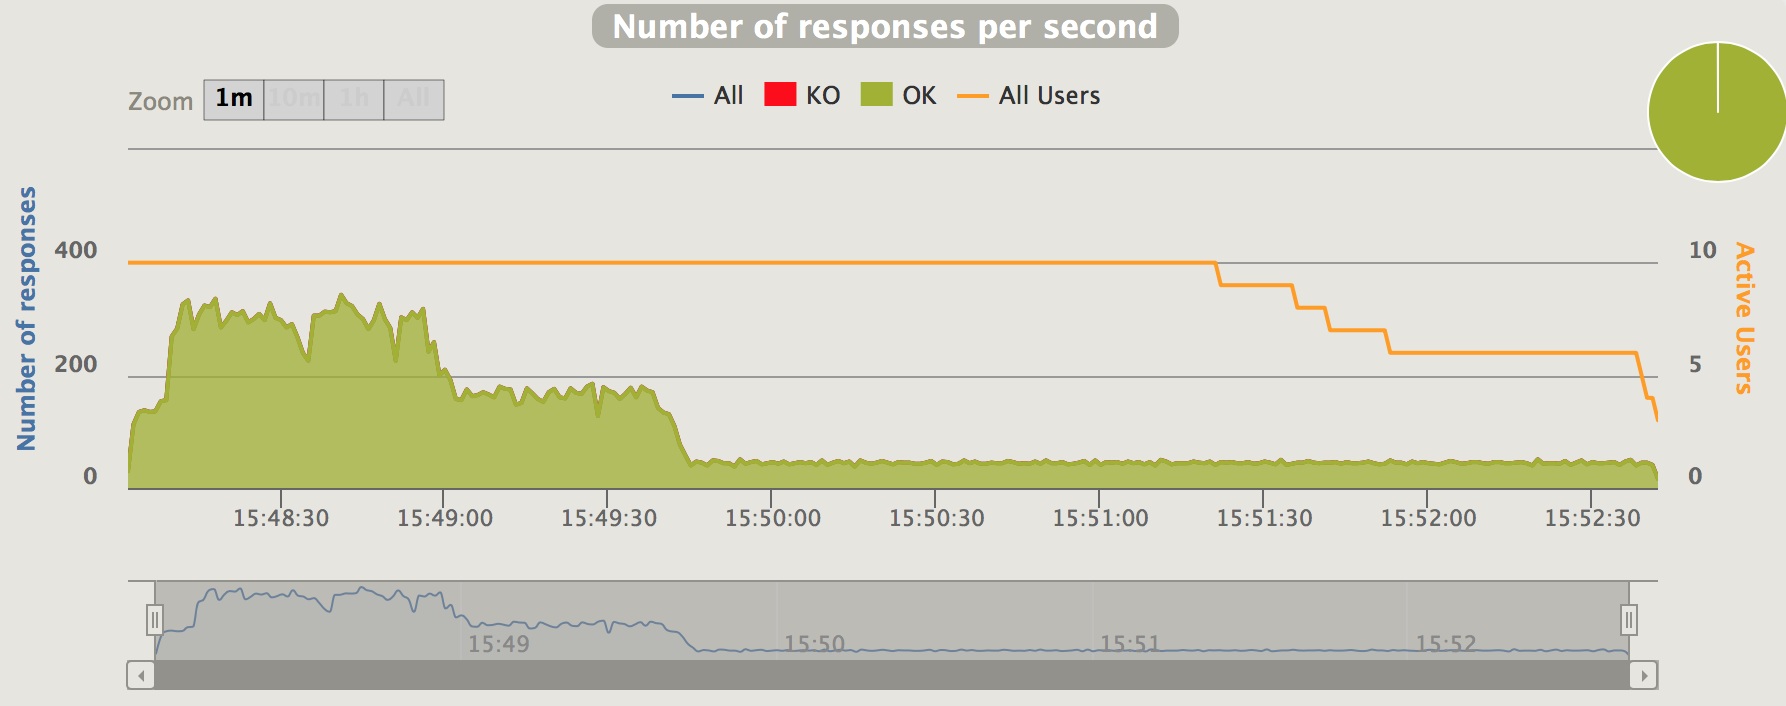
\includegraphics[width=148mm]{images/request}
\caption{并发请求数量}
\label{request}
\end{figure}

\section{后续工作}
1. 修复系统中现存的问题,提高平台稳定性
2. 实现分享功能,可以在用户间分享结构脑图谱,便于用户之间交流
3. 根据压力测试结果,分析系统性能的瓶颈,提升系统性能
4. 撰写毕业论文

\bibliographystyle{data/gbt7714-2005}
{
\renewcommand{\chapter}[2]{\section*{#2}\addcontentsline{toc}{section}{#2}}
\bibliography{data/zhongqi}
}